\documentclass[%
%reprint,
%superscriptaddress,
%groupedaddress,
%unsortedaddress,
%runinaddress,
%frontmatterverbose, 
%preprint,
%showpacs,preprintnumbers,
%nofootinbib,
%nobibnotes,
%bibnotes,
amsmath,amssymb,
%aps,
%pra,
%prb,
%rmp,
%prstab,
%prstper,
%floatfix,
onecolumn,
a4paper,
10pt
]{article}%revtex4-1}

\usepackage{graphicx}% Include figure files
\usepackage{dcolumn}% Align table columns on decimal point
\usepackage{bm}% bold math
\usepackage{titlesec}
%\usepackage[acronym,nomain]{glossaries}
\usepackage[toc,acronym,nomain]{glossaries-prefix}
\usepackage{wrapfig}
%\usepackage[colorlinks]{hyperref}% add hypertext capabilities
\usepackage{hyperref}% add hypertext capabilities
\usepackage[numbers]{natbib}
\usepackage{authblk}
\usepackage{floatrow}
\usepackage[font={small}]{caption}
\usepackage{subcaption}
\usepackage{textcomp}

\hypersetup{colorlinks=true, urlcolor=blue}

%\usepackage[mathlines]{lineno}% Enable numbering of text and display math
%\linenumbers\relax % Commence numbering lines

% Page geometry
\usepackage[
%showframe,
%scale=0.7, marginratio={1:1, 2:3}, ignoreall,% default settings
text={7in,10in},
%centering,
margin=1.5in,
total={8in,10in}, top=1.2in, left=0.9in, bottom=0.75in, includefoot,
height=10in,a4paper,hmargin={3cm,0.8in},
]{geometry}

% Spacing after and before titles
%\titlespacing*{\section}
%{0pt}{5.5ex plus 1ex minus .2ex}{2.3ex plus .2ex}
%\titlespacing*{\subsection}
%{0pt}{5.5ex plus 1ex minus .2ex}{1.3ex plus .2ex}

% Format of sections
\renewcommand\thesection{\arabic{section}}
\renewcommand\thesubsection{\thesection.\arabic{subsection}}
\renewcommand\thesubsubsection{\thesubsection.\arabic{subsubsection}}

% Graphics
\graphicspath{ {../images/} }

% Commands
\newcommand{\quotes}[1]{``#1''}

% New list method
\newlength{\bulletwidth}\settowidth{\bulletwidth}{$\bullet$}
\newcommand{\mitem}{\setlength{\leftskip}{\leftmargin}\hspace*{-\labelsep}\hspace*{-\bulletwidth}$\bullet$\hspace*{\labelsep}}
\newcommand{\mend}{\setlength{\leftskip}{0cm}}
\newcommand{\utilde}{\raise.17ex\hbox{$\scriptstyle\mathtt{\sim}$}}

% abbreviations:
\newcommand*\glsr[2][]{\glsdisp[#1]{#2}{\glsentryshort{#2} (\glsentrylong{#2})}}
\newcommand*\glsrpl[2][]{\glsdisp[#1]{#2}{\glsentryshortpl{#2} (\glsentrylongpl{#2})}}
\newacronym{fwhm}{FWHM}{Full Width at Half Maximum}
\newacronym{vhe}{VHE}{Very High Energy}
\newacronym{psf}{PSF}{Point Spread Function}
\newacronym[prefix={an~}]{nsb}{NSB}{Night-Sky Background}
\newacronym{pe}{p.e.}{Photo-Electron}
\newacronym{adc}{ADC}{Analogue-to-Digital Converter}
\newacronym{pde}{PDE}{Photon Detection Efficiency}
\newacronym{spe}{SPE}{Single Photo-Electron}
\newacronym{eso}{ESO}{European Southern Observatory}
\newacronym{hawc}{HAWC}{High-Altitude Water Cherenkov Observatory}
\newacronym{iact}{IACT}{Imaging Atmospheric Cherenkov Telescope}
\newacronym{hess}{H.E.S.S.}{High Energy Stereoscopic System}
\newacronym{magic}{MAGIC}{Major Atmospheric Gamma Imaging Cherenkov Telescopes}
\newacronym{veritas}{VERITAS}{Very Energetic Radiation Imaging Telescope Array System}
\newacronym[prefixfirst={the~}]{cta}{CTA}{Cherenkov Telescope Array}
\newacronym{lst}{LST}{Large Size Telescope}
\newacronym{mst}{MST}{Medium Size Telescope}
\newacronym{sst}{SST}{Small Size Telescope}
\newacronym[prefixfirst={the~}]{gct}{GCT}{Gamma-ray Cherenkov Telescope}
\newacronym[prefixfirst={the~}]{chec}{CHEC}{Compact High Energy Camera}
\newacronym[prefixfirst={the~}]{chec-m}{CHEC-M}{\gls{chec} using \glspl{mapmt} as the detector}
\newacronym[prefixfirst={the~}]{chec-s}{CHEC-S}{\gls{chec} using \glspl{sipmt} as the detector}
\newacronym{mapmt}{MAPMT}{Multi-Anode Photomultiplier Tube}
\newacronym{sipmt}{SiPMT}{Silicon Photomultiplier Tube}
\newacronym{asic}{ASIC}{Application-Specific Integrated Circuit}
\newacronym{target}{TARGET5}{TeV Array Readout with GSa/s sampling and Event Trigger(version 5)}
\newacronym{fpga}{FPGA}{Field-Programmable Gate Array}
\newacronym{adc2pe}{adc2pe}{conversion of \gls{adc} counts to \gls{pe}}
\newacronym{mc}{MC}{Monte-Carlo}
\newacronym{corsika}{CORSIKA}{COsmic Ray SImulations for KAscade}
\newacronym{hv}{HV}{High Voltage}
\newacronym{impact}{ImPACT}{Image Pixel-wise fit for Atmospheric Cherenkov Telescopes}
% Nomenclature:
%\newglossaryentry{angelsperarea}{
%	name = $a$ ,
%	description = The number of angels per unit area,
%}


\makeglossaries
\begin{document}
	
	\title{Calibration and Analysis of the GCT Camera for the Cherenkov Telescope Array}
	\author{Jason Watson\\\small Supervisor: Dr. Garret Cotter}
	\affil{Department of Astrophysics, University of Oxford, Denys Wilkinson Building, Keble Road, Oxford OX1 3RH, UK}
	%\affiliation{Department of Ast\usepackage{authblk}rophysics, University of Oxford, Denys Wilkinson Building, Keble Road, Oxford OX1 3RH, UK}
	%\collaboration{Supervisor: Dr. Garret Cotter}%\noaffiliation
	\date{\today}
	
	\maketitle
	
	\begin{abstract}
		abstract
	\end{abstract}
	
	\tableofcontents
	
	\clearpage
	
	\section{Introduction}
		\begin{itemize}
			\item High Energy Astrophysics: The universe and 
		\end{itemize}
	
		\textit{With a view to it forming the Introduction to my thesis, this introductory material is the same as from my first year report.}
		Due to the nature of gamma-rays, astronomy at this wavelength is conducted very differently to all other wavelengths. Typically, telescopes make use of the ability to concentrate a rain of photons through reflection or refraction to a photon detector. But as you approach the energies of gamma-rays (100 keV - $>$100 EeV) it becomes extremely inefficient to focus the photons \citep[p.~6]{weekes2003}. Additionally, the atmosphere is effectively opaque to all energies above 10 eV. Therefore in order to detect gamma-rays we need to send a detector into space. The Fermi Large Area Telescope is the latest of gamma-ray detectors in space, and has the dimensions 1.8 m × 1.8 m × 0.72 m, with an effective area at normal incidence of 0.95 meters squared \citep{Atwood2009}. A third difficulty exists in the low flux of cosmic gamma-rays, which decreases further at higher energies, thus requiring a larger collection area. This makes space telescopes impractical for the extremely high energies (TeV) forcing us to use an alternative technique.
		
		There exists a \quotes{gamma-ray window} in the atmosphere. Not in the conventional meaning of transparency, but instead a region in energy from about 100 GeV to 50 TeV \citep[p.~13]{weekes2003}, within which the secondary products of the gamma-ray's interaction with the atmosphere can be detected and used for astronomy. This is known as the \gls{iact} technique.
		
	\begin{figure}
		\centering
		\begin{subfigure}[b]{0.4\textwidth}
			\includegraphics[width=\linewidth]{../images/stereoscopic_technique2}
			\caption{\label{fig:stereoscopic_technique2} An example of combining images of a shower from a stereoscopic system of telescopes.}
		\end{subfigure}
		~
		\begin{subfigure}[b]{0.4\textwidth}
			\includegraphics[width=\textwidth]{../images/hadron_shower}
			\caption{\label{fig:hadron_shower} The difference in shape between a gamma-ray-induced shower (top), and a proton-induced shower (bottom).}
		\end{subfigure}
		\caption{Illustrations of atmospheric Cherenkov showers.}
	\end{figure}		
	
	\subsection{Imaging Atmospheric Cherenkov Technique}
	
	Once a gamma-ray enters the atmosphere, it interacts with the Coulomb field of an atmospheric particle to produce an electron-positron pair. These leptons are highly energetic and will travel superluminally, thereby emitting Cherenkov photons. As they continue further through the atmosphere, they lose energy through Bremsstrahlung, and produce further gamma-rays which can go on the repeat the same process (\autoref{fig:showers}). The absolute outcome is a particle shower starting at around 20 km altitude (due to the radiation length of the atmosphere) continuing as a tight bunch in the original gamma-ray's direction. The number of electrons, positrons and gamma-rays continue to increase until the average energy has dropped to the point where ionisation energy losses become equal to radiation losses. This point is the \quotes{shower maximum}, and afterwards the number of particles gradually diminish, and the shower dies away. The distance the cascade travels depends on the initial gamma energy, but a typical altitude reached is shown in the bottom of \autoref{fig:showers}.

	\begin{figure}
		\centering
		\includegraphics[width=0.4\linewidth]{../images/showers}
		\caption{\label{fig:showers}\textbf{Top-left:} A simple diagram of the nuclear processes occurring in the gamma-ray-induced particle shower's development. Note: the $\gamma$ represent secondary gamma-rays, not Cherenkov photons. \\
			\textbf{Top-right:} A similar diagram for a cosmic-ray-induced particle shower. \\
			\textbf{Bottom:} Schematic of the showers shower the typical altitudes of their developments. \\
			Source: \citep[p.~16]{weekes2003}}
	\end{figure}

	The Cherenkov light from the cascade produces a pool of light with an area of around 0.1 km$^2$ that lasts for around 10 nanoseconds. This optical Cherenkov light is then imaged by an \gls{iact}, where it will see the outline of the shower producing the light (\autoref{fig:cta_shower}). However, in order to see this light among the \gls{nsb}, the telescope is required to operate on nanosecond time-scales with a very fast trigger.
	
	\begin{figure}
		\centering
		\includegraphics[width=0.6\linewidth]{../images/cta_shower}
		\caption{\label{fig:cta_shower}Properties of the Cherenkov light.}
	\end{figure}

	As shown in \autoref{fig:showers}, cosmic-rays (e.g. protons) also produce particle showers. These are $10^3$ - $10^4$ times more common than gamma-ray showers, and are often produced by the similar processes that created the gamma-rays, however they are often undesired for investigating these objects and processes. As cosmic-rays consist of charged particles, they will likely be deflected in their journey to Earth by magnetic fields, and thereby cannot be traced back to their source. We must therefore find techniques with which we can reject this background. Typical techniques involve the exploitation of the different shape between a gamma shower and a proton shower, which can be seen in \autoref{fig:hadron_shower}. A cosmic-ray shower is wider, less tidy, and can sometimes contain ring-like features known as \quotes{muon rings}, produced by a muon penetrating to much lower altitudes while still emitting Cherenkov light.
	
	By tracing back the direction of shower from the image, or a combination of images in a stereoscopic system of telescopes (\autoref{fig:stereoscopic_technique2}), you can locate the origin of the gamma-ray in order to map sources on a celestial sphere. Additionally, since Cherenkov light is emitted from all of the particles of the shower, the atmosphere acts vaguely like a calorimeter, where the amount of Cherenkov light is directly proportional to the energy of the initial gamma-ray. These properties allow the \gls{iact} technique to be used for astronomy. 
	
	\subsection{Cherenkov Telescope Array}
		The application of the \gls{iact} technique was first attempted in the 1960s, but the first large optical refletor built with the purpose of gamma-ray astronomy was the Whipple 10 m telescope in southern Arizona, 1968. At first, gamma-ray astronomy was polluted with unsubstantial claims of transient signals from a variety of pulsars and binaries, but these signals had marginal statistical significance \citep[p.~9]{weekes2003}. It wasn't until 20 years later, after further development of the technique, that the Crab Nebula was detected by Whipple in 1989, thus reigniting interest in the development of gamma-ray astronomy.
		
		Modern \glspl{iact} include \glsr{magic}, \glsr{veritas}, and the most recent, \glsr{hess} (\autoref{fig:iacts}). All three of these telescope systems operate with the advantages of stereoscopic collaboration, allowing multiple images of the same shower to be obtained. In order to improve on the current \glspl{iact}, an array of \utilde100 telescopes was proposed, called \pgls{cta}. This array will have 10 times the sensitivity \gls{hess}, will be able to observe within the energy range 30 GeV - 100 TeV, has a large (\utilde8\textdegree) field of view for surveys, improved angular and energy resolution, and will be the first \gls{iact} to operate as an open observatory \citep{Acharya2013}.
		\begin{figure}[H]
			\centering
			\begin{subfigure}[b]{0.35\textwidth}
				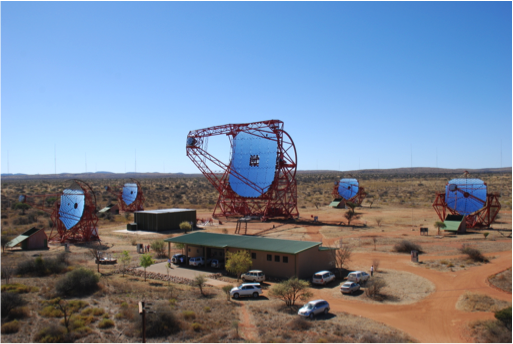
\includegraphics[width=\textwidth]{../images/hess}
				\caption{\gls{hess}}
				\label{fig:hess}
			\end{subfigure}
			~
			\begin{subfigure}[b]{0.35\textwidth}
				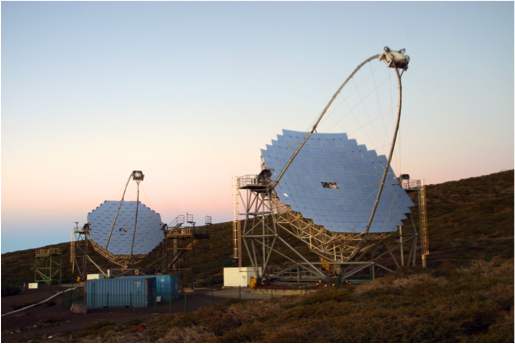
\includegraphics[width=\textwidth]{../images/magic}
				\caption{\gls{magic}}
				\label{fig:magic}
			\end{subfigure}
			~
			\begin{subfigure}[b]{0.45\textwidth}
				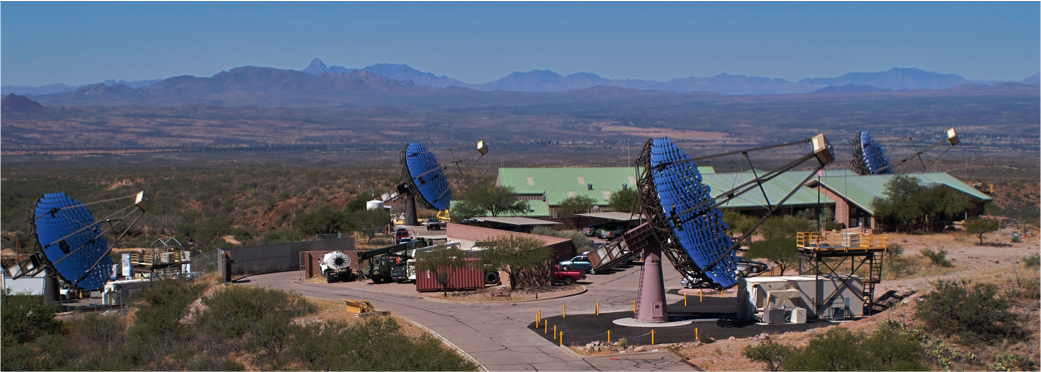
\includegraphics[width=\textwidth]{../images/veritas}
				\caption{\gls{veritas}}
				\label{fig:veritas}
			\end{subfigure}
			\caption{\label{fig:iacts} Pictures of modern \glspl{iact}}
		\end{figure}
		
		\Pgls{cta} will consist of 3 different sized telescopes. For detection of the lower energies below 100 GeV there will be around 4 \glspl{lst} with a mirror diameter of about 23 m in order to collect as many photons as possible from the low energy shower. The mid-range 0.1-10 TeV will be covered by around 25 \glspl{mst} with mirror diameters of 12 m. Finally, the high energies at greater than 10 TeV will be monitored by around 70 \glspl{sst} with mirror diameters of around 4 m. Due to the rarity of higher energy showers, the \glspl{sst} need to be spread over an area of several square kilometres, to increase the chance of a detection \citep{Acharya2013}.
		
		\begin{figure}[H]
			\centering
			\includegraphics[width=0.7\linewidth]{../images/sst}
			\caption{\label{fig:sst} The three different designs of the \gls{sst}.}
		\end{figure}
		
		There exists 3 designs of the \gls{sst}: SST-1M (a single mirror design), ASTRI and \pgls{gct} (both being dual-mirror designs). These are shown in \autoref{fig:sst}. I am part of the \pgls{gct} group, which consists of the France-based GATE structure and mirrors, and the UK-based \gls{chec}. It is the development and commissioning of \gls{chec} that is the focus of my D.Phil.  
	
	\subsection{Compact High Energy Camera}
	
		\Pgls{chec} is further divided into two models, the first being \glsr{chec-m}, whose prototype was integrated onto the GATE telescope structure at the Observatoire de Paris-Meudon in November 2015. The second model is \glsr{chec-s}, and is likely to be the model used in the final \gls{gct} design. The purpose of \gls{chec-m} is accordingly a benchmark and a backup - \gls{sipmt} technology is still quite new, whereas the use of traditional photomultipliers is commonplace in \glspl{iact}. However, it is believed \glspl{sipmt} have advanced to a reliable state, and may surpass the performance of \gls{mapmt} technology.
		
		The design of \pgls{chec-m} contains 2048 pixels (32 x 64 pixel modules) and uses the Hamamatsu H10966B \gls{mapmt}. Behind the \gls{mapmt} are four pre-amplifier boards, used to amplify and shape the waveform pulse. This then continues to the \glsr{target} board, where four custom \glspl{asic} are used to digitise a sample per nanosecond, and to perform the 1st level trigger. The signal is then passed to the \gls{fpga} on-board the \gls{target} module, where the data is serialised and stored in a 16~$\mu$s buffer. The entire electronics schematic is shown in \autoref{fig:camera_electronics}, however the majority of my investigations are focussed on the components preceding the backplane.
		
		\begin{figure}
			\centering
			\begin{subfigure}[b]{0.5\textwidth}
				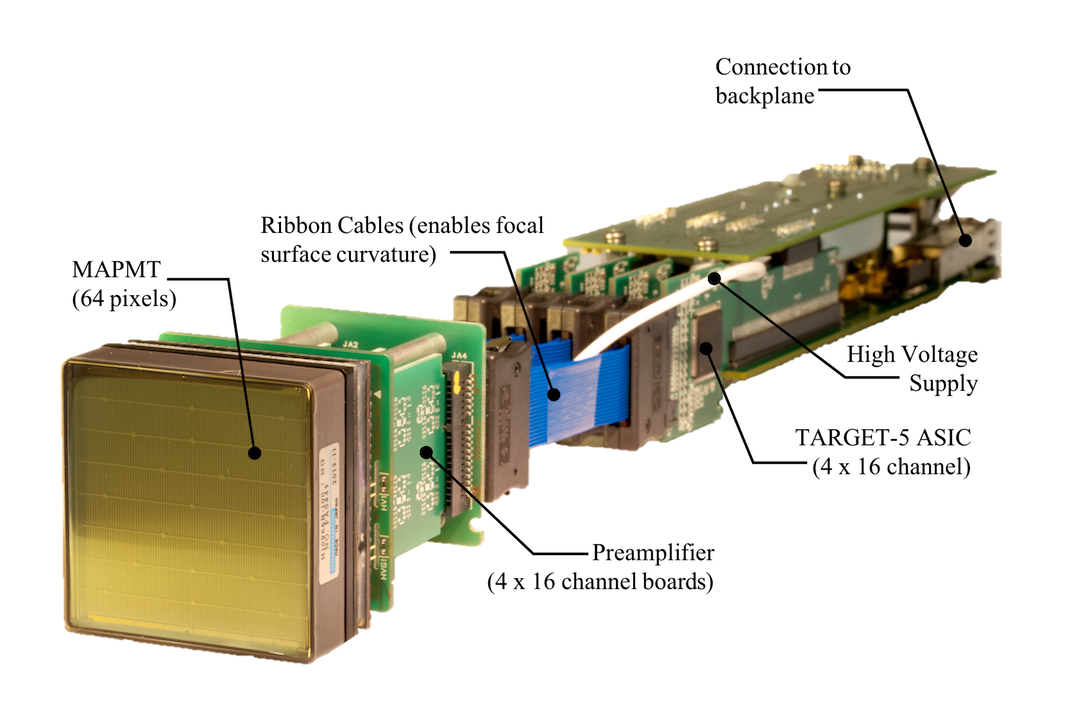
\includegraphics[width=\textwidth]{../images/mapm_module}
				\caption{\gls{mapmt} module.}
				\label{fig:mapm_module}
			\end{subfigure}
			\begin{subfigure}[b]{0.49\textwidth}
				\includegraphics[width=\textwidth]{../images/camera_schematics}
				\caption{Schematics of camera electronics}
				\label{fig:camera_schematics}
			\end{subfigure}
			\caption{\label{fig:camera_electronics} The electronics of \pgls{chec-m}.}
		\end{figure}
	
		\begin{figure}[H]
			\centering
			\includegraphics[width=0.5\linewidth]{../images/lab_setup}
			\caption{The lab set-up for testing the \gls{chec-m} camera at the University of Leicester}
			\label{fig:lab_setup}
		\end{figure}
		
	\section{Commissioning and Inauguration of the First GCT Prototype}
	
	During November 2015, the final tests were conducted with \gls{chec-m} on its workbench in Leicester. This workbench consisted of a light-tight box, within which a laser mounted onto a robot arm would illuminate the entire camera face  (\autoref{fig:lab_setup}). The tests conducted included arrival time calibration from pico-second laser flashes, single-photoelectron measurements for each pixel, gain-matching of all modules, and the determination of transfer-functions for all cells of the four ASICs located on each of the 32 TARGET modules \cite{Brown2016}. Additionally the safety of the camera was evaluated in tests such as temperature control and monitoring. Shown in \autoref{fig:temp} is one of the graphs I produced to display and assess the temperature monitoring performed. These tests concluded that the camera was in a state where it could safely be integrated onto the GATE telescope structure.
	
	\begin{figure}[h]
		\centering
		\includegraphics[width=\linewidth]{../images/temp.png}
		\caption{\label{fig:temp} Visualisation of the temperature monitoring over a 170 minute period, demonstrating our ability to constrain the camera's temperature during normal operation. In the top right is the legend for the graph lines, where ``TM" stands for TARGET module. Shown in the bottom right is the time-averaged temperature distribution across the camera face from 60 to 130 minutes. \cite{Brown2016}}
	\end{figure}
	
	Transported in a shock-absorbent crate, the camera arrived unscathed to Meudon, Paris in mid-November. Upon arrival the camera tests were repeated before installing it onto the telescope structure (\autoref{fig:telescope}). Care was taken in exposing the camera to gradually higher light levels (utilising the camera's lid and the telescope shelter), as this was its first operation outside of a light-tight container, and too high of an exposure would cause irreversible damage to the \glspl{mapmt}.
	
	\begin{figure}[h]
		\captionsetup{type=figure}
		\caption{\label{fig:telescope} The \gls{chec-m} camera mounted onto the GATE telescope structure at the Observatoire de Paris-Meudon.}
		\begin{subfigure}[b]{0.49\textwidth}
			\includegraphics[width=\textwidth]{../images/telescope}
			%		\caption{ }
		\end{subfigure}
		~
		\begin{subfigure}[b]{0.49\textwidth}
			\includegraphics[width=\textwidth]{../images/camera}
			%		\caption{ }
		\end{subfigure}
	\end{figure}
	
	Towards the end of November it was approaching full-moon and there were poor weather conditions, however on the 26th November we were fortunate to have clear skies apart from some cloud blocking the moon. Even with the cloud cover reducing the moonlight, the \gls{nsb} was around 500~MHz, 50 times brighter than the telescope is expected to operate at in the final array. In order to minimise risk the camera was operated with a HV of 750~V, lower than the typical laboratory values of 950~V and 1100~V, consequently only approximate calibration could be applied to any data taken. Additionally the telescope was only fitted with 2 (unaligned) primary mirror petals, while dummies were fitted in the 4 remaining slots. Regardless of these difficulties we proceeded with the observations. My responsibility, aside from guarding the telescope during the observations from passer-byers with torches, was to process the data into some visualisations to be used in the inauguration presentations and proceeding press releases. Shown in \autoref{fig:events} are 6 of the \utilde30 events detected in a total of 10 minutes of observing. These are almost certainly observations of hadron-induced Cherenkov showers, as the telescope had no pointing at the time, and they match the geometry we had predicted with simulations at this \gls{nsb} level. As we store the whole 96~ns waveform when the camera is triggered, we can also perform additional checks on the data. Firstly, the waveforms shown in \autoref{fig:movie} display the expected few nanosecond duration of a Cherenkov shower and occur in a coincident time-window in the relevant pixels. Secondly, the animation from \autoref{fig:movie} shows a movement of the intensity across the camera which is consistent with the signature characteristic of a Cherenkov shower signal \cite{Dournaux2016}.
	
	\newpage
	
	\begin{figure}[H]
		\centering
		\includegraphics[width=0.9\linewidth]{../images/events}
		\caption{\label{fig:events} A selection of the first Cherenkov shower events detected by \gls{chec-m}. The intensity in each pixel is the maximum value of that waveform's pixel after pedestal subtraction. The missing module is a result of a faulty connector on the backplane that has since been replaced. The last event (bottom-right) occurred when the cloud covering the moon reduced, increasing the \glsr{nsb}.}
	\end{figure}
	
	\begin{figure}[hb]
		\centering
		\includegraphics[width=0.9\linewidth]{../images/movie}
		\caption{\label{fig:movie} A frame of an animation showing the progression of the pedestal-subtracted event. The frame coincides with the time of maximum pixel intensity (vertical black line on the waveform). \href{http://www.hap-astroparticle.org/img/news_15-12-08_CTA_GCTPrototype-cam_event_GIF.gif}{The full animation can be found here.}}
	\end{figure}
	
	\newpage
	
	\begin{figure}[H]
		\centering
		\includegraphics[width=0.8\linewidth]{../images/integrator_camera_global}
		\caption{\label{fig:integrator_camera_global} Four displays of a simulated Cherenkov shower event. \textbf{Top-left:} Two examples of which pixels would classify as neighbours to the pixels of interest. \textbf{Top-right:} The camera image at the time-slice of maximum intensity. \textbf{Bottom-left:} The camera image as it would appear from a camera with perfect electronics, showing the exact amount photons that arrive at the camera-face, converted into units of photo-electrons. \textbf{Bottom-right:} The camera image after calibration and waveform integration. This example uses the global-peak integration method.}
	\end{figure}
	
	\begin{figure}[H]
		\centering
		\includegraphics[width=0.7\linewidth]{../images/integrator_waveform_global}
		\caption{\label{fig:integrator_waveform_global} The waveforms for some of the pixels contained in the camera image from \autoref{fig:integrator_camera_global}. The pixels chosen are the ones with highest maximum intensity (and its three neighbours) and the ones with the lowest maximum intensity (and its two neighbours). The red lines illustrate where the integration window was defined for the pixel. The true charge (what you would obtain with perfect electronics) and the measured charge (the result of the integration and calibration) is also displayed in the titles of the waveforms.}
	\end{figure}
	
	\begin{figure}[H]
		\centering
		\includegraphics[width=0.9\linewidth]{../images/integrator_camera_local}
		\caption{\label{fig:integrator_camera_local} Same as \autoref{fig:integrator_camera_global}, but using the local-peak integration method.}
	\end{figure}
	
	\begin{figure}[H]
		\centering
		\includegraphics[width=0.9\linewidth]{../images/integrator_waveform_local}
		\caption{\label{fig:integrator_waveform_local} The waveforms for some of the pixels corresponding to the camera image in \autoref{fig:integrator_camera_local}. The pixels chosen are the same as in \autoref{fig:integrator_waveform_global}}
	\end{figure}
	
	\newpage
	
	\section{Development of CTA Pipeline Software}
	
	Following my work with simulation data in my first year, and the contributions I made to analysis of the first on-sky data, I began to work with the CTA Pipeline Software. This is a Python project intended to hold the full analysis chain of CTA data for all telescopes, accepting both real and simulated data. I was introduced to the pipeline at the first workshop held at DESY (Zeuthen, Berlin), and have continued to participate in its development since then. My main contribution is the calibration pipeline for the simulation data, which was driven by my desire to continue my charge resolution investigations (see first year report) inside the pipeline framework due to the advantages Python provides. One major advantage it has is the ease at which you can probe each process of the code, and easily create plots to check it functions as expected. \autoref{fig:integrator_camera_global} displays the camera image as a result of the global-peak integration method, which performs a weighted average of the time-of-maximum-intensity for each pixel with the aim to find the best time to integrate about. Being able to display the camera image resulting from this integration method alongside other views of the same event, in addition to the examples of integration window (\autoref{fig:integrator_waveform_global}), clearly suggests that the method may not be useful. Had only the final calibrated image been shown (bottom right of \autoref{fig:integrator_camera_global}) it may not have been apparent that there was a failure in the integration method. \autoref{fig:integrator_camera_local} shows the same event, but using the local-peak integration method, where the integration widow is defined independently for each pixel based of its own time-of-maximum-intensity (\autoref{fig:integrator_waveform_local}). It is clear from the calibrated image and the waveforms that this is a more successful method of integration.
		
	\section{Future}
	In addition to the continuation of my previously described activities, I will adopt the following investigations during my D.Phil.
	
	\subsection{GCT Calibration inside the CTA Pipeline}
	Currently, the data storage format for CTA telescopes has not been defined. This makes it difficult to extend the analysis of GCT data into the CTA Pipeline. Therefore I developed a Python module that utilises a Python wrapper for TargetIO (the C++ library that reads \gls{chec-m} data from a fits file) and pipes it into the event containers used by CTA Pipeline. This allows us to use the pipeline framework on real data, and as \gls{chec-m} is the first working prototype camera, allows us to direct and assist with the Pipeline development. I will continue in this contribution by implementing the calibration of \gls{chec-m} data into the Pipeline, primarily so that we can continue its analysis further, but also to provide an example for other camera teams in CTA so they may easily integrate their own calibration too.
	
	\subsection{ImPACT}
	I have just begun my 6 month visit to the Max-Planck Institute for Nuclear Physics (MPIK) in Heidelberg that was previously mentioned in my first year report. My primary focus during this stay is to further develop the image-reconstruction method \glsr{impact} \citep{Parsons2014}. This technique utilises Monte Carlo simulations of air showers with accurate models of the telescope optics and electronics to produce templates of camera images with known shower properties (e.g. Energy, Direction). Real camera images can then be compared against them using a log-likelihood method to accurately reconstruct the real shower's properties. Currently the technique is only applied to the pixel intensity images, with no consideration of the time-development of individual showers. This time information contains useful discriminating properties, and is retained in the stored waveforms of our camera data. Therefore utilising this information in the \gls{impact} technique could greatly increase its success in shower reconstruction.
	
	\subsection{On-sky Data Analysis}
	The second on-sky campaign for the \gls{gct} prototype will occur in October 2016, where \gls{chec-m} will be transported from its new lab at the MPIK back to the Observatoire de Paris-Meudon. This is unlikely to be the final campaign during my D.Phil - there are plans to integrate \gls{chec-m} onto an ASTRI telescope structure during 2017, in accordance with the original design of the camera mechanics. During one of these campaigns we intend to attempt an observation of an astronomical gamma-ray source such as the Crab Nebula. Following my previous handling of the camera data, I have been tasked with the analysis of such scientific data, with which I will attempt to produce an image and energy spectrum of the source. This will be the first astronomical analysis performed with a \gls{cta} prototype.
	
	\subsection{Catalogue Searches}
	In the unfortunate circumstance that no astronomical source is observed with the \gls{gct} prototype, I have prepared a backup plan to perform a scientific investigation using an existing gamma-ray source catalogue.  This will likely be the \textit{Fermi} 4-year point source catalogue (3FGL) \cite{Acero2015}, which is publicly available. Novel source detection algorithms tailored specifically to gamma-ray astronomy are under development, such as that of Armstrong el al.\cite{Armstrong2015a} using clustering algorithms. I would develop this, looking specifically at the CTA sky surveys, to provide a data-based thesis chapter if the telescope on-sky data is delayed.
	
	\bibliographystyle{../bibtex/unsrt_j}%../bibtex/apa-good}
	\bibliography{../bibtex/papers,../bibtex/books,../bibtex/websites}
	
	\newpage
	\printglossary[nonumberlist,type=\acronymtype,title=Abbreviations]

\end{document}
